% Options for packages loaded elsewhere
\PassOptionsToPackage{unicode}{hyperref}
\PassOptionsToPackage{hyphens}{url}
%
\documentclass[
]{article}
\usepackage{lmodern}
\usepackage{amssymb,amsmath}
\usepackage{ifxetex,ifluatex}
\ifnum 0\ifxetex 1\fi\ifluatex 1\fi=0 % if pdftex
  \usepackage[T1]{fontenc}
  \usepackage[utf8]{inputenc}
  \usepackage{textcomp} % provide euro and other symbols
\else % if luatex or xetex
  \usepackage{unicode-math}
  \defaultfontfeatures{Scale=MatchLowercase}
  \defaultfontfeatures[\rmfamily]{Ligatures=TeX,Scale=1}
\fi
% Use upquote if available, for straight quotes in verbatim environments
\IfFileExists{upquote.sty}{\usepackage{upquote}}{}
\IfFileExists{microtype.sty}{% use microtype if available
  \usepackage[]{microtype}
  \UseMicrotypeSet[protrusion]{basicmath} % disable protrusion for tt fonts
}{}
\makeatletter
\@ifundefined{KOMAClassName}{% if non-KOMA class
  \IfFileExists{parskip.sty}{%
    \usepackage{parskip}
  }{% else
    \setlength{\parindent}{0pt}
    \setlength{\parskip}{6pt plus 2pt minus 1pt}}
}{% if KOMA class
  \KOMAoptions{parskip=half}}
\makeatother
\usepackage{xcolor}
\IfFileExists{xurl.sty}{\usepackage{xurl}}{} % add URL line breaks if available
\IfFileExists{bookmark.sty}{\usepackage{bookmark}}{\usepackage{hyperref}}
\hypersetup{
  pdftitle={Machine Learning - Block 01 Lab 2 - Exam Prep},
  pdfauthor={Agustín Valencia},
  hidelinks,
  pdfcreator={LaTeX via pandoc}}
\urlstyle{same} % disable monospaced font for URLs
\usepackage[margin=1in]{geometry}
\usepackage{color}
\usepackage{fancyvrb}
\newcommand{\VerbBar}{|}
\newcommand{\VERB}{\Verb[commandchars=\\\{\}]}
\DefineVerbatimEnvironment{Highlighting}{Verbatim}{commandchars=\\\{\}}
% Add ',fontsize=\small' for more characters per line
\usepackage{framed}
\definecolor{shadecolor}{RGB}{248,248,248}
\newenvironment{Shaded}{\begin{snugshade}}{\end{snugshade}}
\newcommand{\AlertTok}[1]{\textcolor[rgb]{0.94,0.16,0.16}{#1}}
\newcommand{\AnnotationTok}[1]{\textcolor[rgb]{0.56,0.35,0.01}{\textbf{\textit{#1}}}}
\newcommand{\AttributeTok}[1]{\textcolor[rgb]{0.77,0.63,0.00}{#1}}
\newcommand{\BaseNTok}[1]{\textcolor[rgb]{0.00,0.00,0.81}{#1}}
\newcommand{\BuiltInTok}[1]{#1}
\newcommand{\CharTok}[1]{\textcolor[rgb]{0.31,0.60,0.02}{#1}}
\newcommand{\CommentTok}[1]{\textcolor[rgb]{0.56,0.35,0.01}{\textit{#1}}}
\newcommand{\CommentVarTok}[1]{\textcolor[rgb]{0.56,0.35,0.01}{\textbf{\textit{#1}}}}
\newcommand{\ConstantTok}[1]{\textcolor[rgb]{0.00,0.00,0.00}{#1}}
\newcommand{\ControlFlowTok}[1]{\textcolor[rgb]{0.13,0.29,0.53}{\textbf{#1}}}
\newcommand{\DataTypeTok}[1]{\textcolor[rgb]{0.13,0.29,0.53}{#1}}
\newcommand{\DecValTok}[1]{\textcolor[rgb]{0.00,0.00,0.81}{#1}}
\newcommand{\DocumentationTok}[1]{\textcolor[rgb]{0.56,0.35,0.01}{\textbf{\textit{#1}}}}
\newcommand{\ErrorTok}[1]{\textcolor[rgb]{0.64,0.00,0.00}{\textbf{#1}}}
\newcommand{\ExtensionTok}[1]{#1}
\newcommand{\FloatTok}[1]{\textcolor[rgb]{0.00,0.00,0.81}{#1}}
\newcommand{\FunctionTok}[1]{\textcolor[rgb]{0.00,0.00,0.00}{#1}}
\newcommand{\ImportTok}[1]{#1}
\newcommand{\InformationTok}[1]{\textcolor[rgb]{0.56,0.35,0.01}{\textbf{\textit{#1}}}}
\newcommand{\KeywordTok}[1]{\textcolor[rgb]{0.13,0.29,0.53}{\textbf{#1}}}
\newcommand{\NormalTok}[1]{#1}
\newcommand{\OperatorTok}[1]{\textcolor[rgb]{0.81,0.36,0.00}{\textbf{#1}}}
\newcommand{\OtherTok}[1]{\textcolor[rgb]{0.56,0.35,0.01}{#1}}
\newcommand{\PreprocessorTok}[1]{\textcolor[rgb]{0.56,0.35,0.01}{\textit{#1}}}
\newcommand{\RegionMarkerTok}[1]{#1}
\newcommand{\SpecialCharTok}[1]{\textcolor[rgb]{0.00,0.00,0.00}{#1}}
\newcommand{\SpecialStringTok}[1]{\textcolor[rgb]{0.31,0.60,0.02}{#1}}
\newcommand{\StringTok}[1]{\textcolor[rgb]{0.31,0.60,0.02}{#1}}
\newcommand{\VariableTok}[1]{\textcolor[rgb]{0.00,0.00,0.00}{#1}}
\newcommand{\VerbatimStringTok}[1]{\textcolor[rgb]{0.31,0.60,0.02}{#1}}
\newcommand{\WarningTok}[1]{\textcolor[rgb]{0.56,0.35,0.01}{\textbf{\textit{#1}}}}
\usepackage{graphicx}
\makeatletter
\def\maxwidth{\ifdim\Gin@nat@width>\linewidth\linewidth\else\Gin@nat@width\fi}
\def\maxheight{\ifdim\Gin@nat@height>\textheight\textheight\else\Gin@nat@height\fi}
\makeatother
% Scale images if necessary, so that they will not overflow the page
% margins by default, and it is still possible to overwrite the defaults
% using explicit options in \includegraphics[width, height, ...]{}
\setkeys{Gin}{width=\maxwidth,height=\maxheight,keepaspectratio}
% Set default figure placement to htbp
\makeatletter
\def\fps@figure{htbp}
\makeatother
\setlength{\emergencystretch}{3em} % prevent overfull lines
\providecommand{\tightlist}{%
  \setlength{\itemsep}{0pt}\setlength{\parskip}{0pt}}
\setcounter{secnumdepth}{-\maxdimen} % remove section numbering
% https://github.com/rstudio/rmarkdown/issues/337
\let\rmarkdownfootnote\footnote%
\def\footnote{\protect\rmarkdownfootnote}

% https://github.com/rstudio/rmarkdown/pull/252
\usepackage{titling}
\setlength{\droptitle}{-2em}

\pretitle{\vspace{\droptitle}\centering\huge}
\posttitle{\par}

\preauthor{\centering\large\emph}
\postauthor{\par}

\predate{\centering\large\emph}
\postdate{\par}

\title{Machine Learning - Block 01 Lab 2 - Exam Prep}
\author{Agustín Valencia}
\date{12/5/2019}

\begin{document}
\maketitle

\hypertarget{assignment-1.-lda-and-logistic-regression}{%
\section{Assignment 1. LDA and logistic
regression}\label{assignment-1.-lda-and-logistic-regression}}

The data file australian-crabs.csv contains measurements of various
crabs, such as frontal lobe, rear width and others.

\begin{enumerate}
\def\labelenumi{\arabic{enumi}.}
\tightlist
\item
  Use australian-crabs.csv and make a scatterplot of carapace length
  (CL) versus rear width (RW) where observations are colored by sex. Do
  you think that this data is easy to classify by linear discriminant
  analysis? Motivate your answer.
\end{enumerate}

Plotting the data

\begin{Shaded}
\begin{Highlighting}[]
\NormalTok{data <{-}}\StringTok{ }\KeywordTok{read.csv2}\NormalTok{(}\StringTok{"data/australian{-}crabs.csv"}\NormalTok{, }\DataTypeTok{sep =} \StringTok{","}\NormalTok{, }\DataTypeTok{dec=}\StringTok{"."}\NormalTok{)}
\NormalTok{males <{-}}\StringTok{ }\NormalTok{data[}\KeywordTok{which}\NormalTok{(data}\OperatorTok{$}\NormalTok{sex }\OperatorTok{==}\StringTok{ "Male"}\NormalTok{),]}
\NormalTok{females <{-}}\StringTok{ }\NormalTok{data[}\KeywordTok{which}\NormalTok{(data}\OperatorTok{$}\NormalTok{sex }\OperatorTok{==}\StringTok{ "Female"}\NormalTok{),]}
\KeywordTok{ggplot}\NormalTok{() }\OperatorTok{+}\StringTok{ }\KeywordTok{ggtitle}\NormalTok{(}\StringTok{"Carapace length vs Rear width by sex"}\NormalTok{) }\OperatorTok{+}
\StringTok{    }\KeywordTok{geom\_point}\NormalTok{(}\KeywordTok{aes}\NormalTok{(}\DataTypeTok{y =}\NormalTok{ females}\OperatorTok{$}\NormalTok{CL, }\DataTypeTok{x =}\NormalTok{ females}\OperatorTok{$}\NormalTok{RW, }\DataTypeTok{color =} \StringTok{"Females"}\NormalTok{)) }\OperatorTok{+}
\StringTok{    }\KeywordTok{geom\_point}\NormalTok{(}\KeywordTok{aes}\NormalTok{(}\DataTypeTok{y =}\NormalTok{ males}\OperatorTok{$}\NormalTok{CL, }\DataTypeTok{x =}\NormalTok{ males}\OperatorTok{$}\NormalTok{RW, }\DataTypeTok{color =} \StringTok{"Males"}\NormalTok{)) }\OperatorTok{+}
\StringTok{    }\KeywordTok{xlab}\NormalTok{(}\StringTok{"Rear Width"}\NormalTok{) }\OperatorTok{+}\StringTok{ }\KeywordTok{ylab}\NormalTok{(}\StringTok{"Carapace Length"}\NormalTok{) }
\end{Highlighting}
\end{Shaded}

\includegraphics{ExamPrep_B1A2_files/figure-latex/crab1-1.pdf}

The classes are overlapped that indicates that linear classification is
not easy. Since LDA maximize the separability between classes it might
be a good choice to perform it in order to get a better scenario to
classify these classes.

\begin{enumerate}
\def\labelenumi{\arabic{enumi}.}
\setcounter{enumi}{1}
\tightlist
\item
  Make LDA analysis with target Sex and features CL and RW and
  propostional prior by using \texttt{lda()} function in package
  \texttt{MASS}. Make a scatterplot of CL versus RW colored by the
  predicted Sex and compare it with the plot in step 1. Compute the
  misclassification error and comment on the quality of fit.
\end{enumerate}

\begin{Shaded}
\begin{Highlighting}[]
\NormalTok{ldaModel <{-}}\StringTok{ }\KeywordTok{lda}\NormalTok{( sex }\OperatorTok{\textasciitilde{}}\StringTok{ }\NormalTok{RW }\OperatorTok{+}\StringTok{ }\NormalTok{CL, }\DataTypeTok{data =}\NormalTok{ data)}
\NormalTok{predictions <{-}}\StringTok{ }\KeywordTok{predict}\NormalTok{(ldaModel, data)}
\NormalTok{predictedData <{-}}\StringTok{ }\KeywordTok{data.frame}\NormalTok{(}
\NormalTok{  sex <{-}}\StringTok{ }\NormalTok{predictions}\OperatorTok{$}\NormalTok{class,}
\NormalTok{  CL <{-}}\StringTok{ }\NormalTok{data}\OperatorTok{$}\NormalTok{CL,}
\NormalTok{  RW <{-}}\StringTok{ }\NormalTok{data}\OperatorTok{$}\NormalTok{RW}
\NormalTok{)}
\KeywordTok{ggplot}\NormalTok{() }\OperatorTok{+}\StringTok{ }\KeywordTok{ggtitle}\NormalTok{(}\StringTok{"Sex Classification using LDA : Sex \textasciitilde{} RW + CL"}\NormalTok{) }\OperatorTok{+}
\StringTok{    }\KeywordTok{geom\_point}\NormalTok{(}\KeywordTok{aes}\NormalTok{(}\DataTypeTok{y =}\NormalTok{ predictedData[}\KeywordTok{which}\NormalTok{(sex }\OperatorTok{==}\StringTok{ "Female"}\NormalTok{), ]}\OperatorTok{$}\NormalTok{CL, }
                   \DataTypeTok{x =}\NormalTok{ predictedData[}\KeywordTok{which}\NormalTok{(sex }\OperatorTok{==}\StringTok{ "Female"}\NormalTok{), ]}\OperatorTok{$}\NormalTok{RW, }
                   \DataTypeTok{color =} \StringTok{"Females"}\NormalTok{)) }\OperatorTok{+}
\StringTok{    }\KeywordTok{geom\_point}\NormalTok{(}\KeywordTok{aes}\NormalTok{(}\DataTypeTok{y =}\NormalTok{ predictedData[}\KeywordTok{which}\NormalTok{(sex }\OperatorTok{==}\StringTok{ "Male"}\NormalTok{), ]}\OperatorTok{$}\NormalTok{CL, }
                   \DataTypeTok{x =}\NormalTok{ predictedData[}\KeywordTok{which}\NormalTok{(sex }\OperatorTok{==}\StringTok{ "Male"}\NormalTok{), ]}\OperatorTok{$}\NormalTok{RW, }
                   \DataTypeTok{color =} \StringTok{"Males"}\NormalTok{)) }\OperatorTok{+}
\StringTok{    }\KeywordTok{xlab}\NormalTok{(}\StringTok{"Rear Width"}\NormalTok{) }\OperatorTok{+}\StringTok{ }\KeywordTok{ylab}\NormalTok{(}\StringTok{"Carapace Length"}\NormalTok{) }
\end{Highlighting}
\end{Shaded}

\includegraphics{ExamPrep_B1A2_files/figure-latex/unnamed-chunk-1-1.pdf}

\begin{Shaded}
\begin{Highlighting}[]
\KeywordTok{get\_performance}\NormalTok{(data}\OperatorTok{$}\NormalTok{sex, predictions}\OperatorTok{$}\NormalTok{class, }\StringTok{"Sex classification using LDA"}\NormalTok{)}
\end{Highlighting}
\end{Shaded}

\begin{verbatim}
## Classification Performance : Sex classification using LDA 
## [1] "Confusion Matrix"
##         predictions
## targets  Female Male
##   Female     97    3
##   Male        4   96
## Rates details:
##  TPR = 96.9697 % - TNR = 96.0396 % - FPR = 3.030303 % - FNR = 3.960396 %
##  Misclassification Rate =  3.5 %
\end{verbatim}

Now it can be seen that no classes are overlapped which means that there
are some classification errors.

\hypertarget{assignment-2.-analysis-of-credit-scoring}{%
\section{Assignment 2. Analysis of credit
scoring}\label{assignment-2.-analysis-of-credit-scoring}}

The data file creditscoring.xls contains data retrieved from a database
in a private enterprise. Each row contains information about one
customer. The variable good/bad indicates how the customers have managed
their loans. The other features are potential predictors. Your task is
to derive a prediction model that can be used to predict whether or not
a new customer is likely to pay back the loan.

\begin{enumerate}
\def\labelenumi{\arabic{enumi}.}
\tightlist
\item
  Import the data to R and divide into training/validation/test as
  50/25/25: use data partitioning code specified in Lecture 1e.
\end{enumerate}

\begin{verbatim}
## Data set size        : 1000 20
\end{verbatim}

\begin{verbatim}
## Training set size    : 500 20
\end{verbatim}

\begin{verbatim}
## Validation set size  : 250 20
\end{verbatim}

\begin{verbatim}
## Testing set size     : 250 20
\end{verbatim}

\begin{enumerate}
\def\labelenumi{\arabic{enumi}.}
\setcounter{enumi}{1}
\tightlist
\item
  Fit a decision tree to the training data by using the following
  measures of impurity and report the misclassification rates for the
  training and test data. Choose the measure providing the better
  results for the following steps.
\end{enumerate}

\begin{enumerate}
\def\labelenumi{\alph{enumi}.}
\tightlist
\item
  Deviance
\end{enumerate}

\begin{center}\includegraphics[height=0.3\textheight]{ExamPrep_B1A2_files/figure-latex/q2_tree_deviance-1} \end{center}

\begin{verbatim}
## Classification Performance : Tree. split = deviance 
## [1] "Confusion Matrix"
##        predictions
## targets bad good
##    bad   24   54
##    good  17  155
## Rates details:
##  TPR = 74.16268 % - TNR = 58.53659 % - FPR = 25.83732 % - FNR = 41.46341 %
##  Misclassification Rate =  28.4 %
\end{verbatim}

\begin{enumerate}
\def\labelenumi{\alph{enumi}.}
\setcounter{enumi}{1}
\tightlist
\item
  Gini index
\end{enumerate}

\begin{center}\includegraphics{ExamPrep_B1A2_files/figure-latex/q2_tree_gini-1} \end{center}

\begin{verbatim}
## Classification Performance : Tree. split = gini 
## [1] "Confusion Matrix"
##        predictions
## targets bad good
##    bad   22   56
##    good  32  140
## Rates details:
##  TPR = 71.42857 % - TNR = 40.74074 % - FPR = 28.57143 % - FNR = 59.25926 %
##  Misclassification Rate =  35.2 %
\end{verbatim}

In summary, the tree trained using deviance as split method performs
better than the one using Gini Index given its misclassification rate
and its true positives rate. Also, the one with deviance is considerably
smaller than the Gini one, this size difference might show some grade of
overfitting in the later.

\newpage
3

. Use training and validation sets to choose the optimal tree depth.
Present the graphs of the dependence of deviances for the training and
the validation data on the number of leaves. Report the optimal tree,
report it's depth and the variables used by the tree. Interpret the
information provided by the tree structure. Estimate the
misclassification rate for the test data.

Crossvalidating the deviance-trained tree:

\begin{center}\includegraphics[height=0.4\textheight]{ExamPrep_B1A2_files/figure-latex/q2_devtree_optimal_depth-1} \end{center}

\begin{verbatim}
## The optimal tree is at depth 4 with deviance 282.6919
\end{verbatim}

In the graph above it is shown the deviances scores obtained by pruned
trees for the given depths for both, training and testing data.
Considering testing data as the one in which the selection decision has
to been based on, it can be seen that the optimal depth is 4 in which
the lowest deviance is obtained (282.7)

Said that, the optimal tree is the following:

\begin{center}\includegraphics[height=0.3\textheight]{ExamPrep_B1A2_files/figure-latex/q2_optimal_tree-1} \end{center}

For which the performance under testing data is:

\begin{verbatim}
## Classification Performance : Optimal Tree - test data 
## [1] "Confusion Matrix"
##        predictions
## targets bad good
##    bad   19   59
##    good   6  166
## Rates details:
##  TPR = 73.77778 % - TNR = 76 % - FPR = 26.22222 % - FNR = 24 %
##  Misclassification Rate =  26 %
\end{verbatim}

\begin{enumerate}
\def\labelenumi{\arabic{enumi}.}
\setcounter{enumi}{3}
\tightlist
\item
  Use training data to perform classification using Naïve Bayes and
  report the confusion matrices and misclassification rates for the
  training and for the test data. Compare the results with those from
  step 3.
\end{enumerate}

\begin{verbatim}
## Classification Performance : Naive Bayes - Train 
## [1] "Confusion Matrix"
##        predictions
## targets bad good
##    bad   95   52
##    good  98  255
## Rates details:
##  TPR = 83.06189 % - TNR = 49.2228 % - FPR = 16.93811 % - FNR = 50.7772 %
##  Misclassification Rate =  30 %
\end{verbatim}

\begin{verbatim}
## Classification Performance : Naive Bayes - test 
## [1] "Confusion Matrix"
##        predictions
## targets bad good
##    bad   47   31
##    good  49  123
## Rates details:
##  TPR = 79.87013 % - TNR = 48.95833 % - FPR = 20.12987 % - FNR = 51.04167 %
##  Misclassification Rate =  32 %
\end{verbatim}

Although tree classifier seems to perform better given that it gets the
lowest misclassification rate under testig data, Naïve Bayes classifier
gets better True Positives rate, which, depending on the application of
the predictor, might be more desireable than the other.

For this particular application in which it is desired to get the loans
paid, misclasification could be considered more important, so Tree
classifier is chosen to be deployed.

Overall, none of two outstands in their performance.

\begin{enumerate}
\def\labelenumi{\arabic{enumi}.}
\setcounter{enumi}{4}
\tightlist
\item
  Use the optimal tree and the Naïve Bayes model to classify the test
  data by using the following principle: \(\hat{Y} = 1\) if
  \(p(Y=good|X) > \pi\), otherwise \(\hat{Y}=0\) where
  \(\pi = 0.05, 0.1, 0.15, ..., 0.9, 0.95\). Compute the TPR and FPR
  values for the two models and plot the corresponding ROC curves.
  Conclusion?
\end{enumerate}

Using the given thresholds the following ROC are obtained:

\begin{center}\includegraphics[height=0.4\textheight]{ExamPrep_B1A2_files/figure-latex/q2_roc_curves-1} \end{center}

The blue line represents where the false positive rate is equal than the
true positive rates. As it has been said in the previous question,
though Naïve Bayes seems to show worse misclassification rates, it tends
to get better results regarding true positives and that can be seen on
the ROC curve. At higher thresholds Naîve Bayes seems to perform better
than the tree classifier.

\begin{enumerate}
\def\labelenumi{\arabic{enumi}.}
\setcounter{enumi}{5}
\tightlist
\item
  Repeat Naïve Bayes classification as it was in step 4 but use the
  following loss matrix.
\end{enumerate}

\begin{center}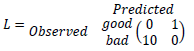
\includegraphics[height=0.1\textheight]{img/loss_matrix} \end{center}

and report the confusion matrix for the training and test data. Compare
the results with the results from step 4 and discuss how the rates have
changed and why.

\begin{verbatim}
## [1] "Loss Matrix"
\end{verbatim}

\begin{verbatim}
##      [,1] [,2]
## [1,]    0    1
## [2,]   10    0
\end{verbatim}

\begin{verbatim}
## Classification Performance : Naive Bayes new rule - Training 
## [1] "Confusion Matrix"
##        predictions
## targets good bad
##    bad    27 120
##    good   17 336
## Rates details:
##  TPR = 73.68421 % - TNR = 61.36364 % - FPR = 26.31579 % - FNR = 38.63636 %
##  Misclassification Rate =  27.4 %
\end{verbatim}

\begin{verbatim}
## Classification Performance : Naive Bayes new rule - Test 
## [1] "Confusion Matrix"
##        predictions
## targets good bad
##    bad    13  65
##    good    7 165
## Rates details:
##  TPR = 71.73913 % - TNR = 65 % - FPR = 28.26087 % - FNR = 35 %
##  Misclassification Rate =  28.8 %
\end{verbatim}

The new loss matrix penalizes ten times more the false positives, then
misclassification rates are lower than before.

\hypertarget{assignment-3-uncertainty-estimation}{%
\section{Assignment 3 : Uncertainty
estimation}\label{assignment-3-uncertainty-estimation}}

The data file State.csv contains per capita state and local public
expenditures and associated state demographic and economic
characteristics, 1960, and there are variables

\begin{itemize}
\tightlist
\item
  MET: Percentage of population living in standard metropolitan areas
\item
  EX: Per capita state and local public expenditures (\$)
\end{itemize}

\begin{enumerate}
\def\labelenumi{\arabic{enumi}.}
\item
  Reorder your data with respect to the increase of MET and plot EX
  versus MET. Discuss what kind of model can be appropriate here. Use
  the reordered data in steps 2-5.
\item
  Use package tree and fit a regression tree model with target EX and
  feature MET in which the number of the leaves is selected by
  cross-validation, use the entire data set and set minimum number of
  observations in a leaf equal to 8 (setting minsize in tree.control).
  Report the selected tree. Plot the original and the fitted data and
  histogram of residuals. Comment on the distribution of the residuals
  and the quality of the fit.
\end{enumerate}

\begin{center}\includegraphics[height=0.4\textheight]{ExamPrep_B1A2_files/figure-latex/q3_tree_train-1} \end{center}

Finding the optimal tree using crossvalidation:

\begin{center}\includegraphics[height=0.4\textheight]{ExamPrep_B1A2_files/figure-latex/q3_tree_plot-1} \end{center}

It can be observed that the optimal tree performance is at size=3.
Pruning the tree to fit that it is obtained the following tree:

\begin{center}\includegraphics[height=0.3\textheight]{ExamPrep_B1A2_files/figure-latex/q3_tree_prune-1} \end{center}

Comparing the predictions made by the optimal tree against the actual
data:

\begin{center}\includegraphics[height=0.4\textheight]{ExamPrep_B1A2_files/figure-latex/q3_tree_predictions-1} \end{center}

And analyzing the residuals for the shown predictions:

\begin{center}\includegraphics[height=0.4\textheight]{ExamPrep_B1A2_files/figure-latex/q3_tree_residuals-1} \end{center}

\begin{verbatim}
## Residuals mean: 1.18525e-14
\end{verbatim}

\begin{verbatim}
## Residuals variance: 2582.858
\end{verbatim}

While visualy analizing the residuals it seems to follow a bell curve
skewed to the right, though when checking the statistics from them it
can be seen that its mean is close to zero and have a huge variance.
Given the little amount of data it is not simple to argue a certain
distribution, so it is recommended to assume a Gaussian distribution
with mean zero.

\begin{enumerate}
\def\labelenumi{\arabic{enumi}.}
\setcounter{enumi}{2}
\tightlist
\item
  Compute and plot the 95\% confidence bands for the regression tree
  model from step 2 (fit a regression tree with the same settings and
  the same number of leaves as in step 2 to the resampled data) by using
  a non-parametric bootstrap. Comment whether the band is smooth or
  bumpy and try to explain why. Consider the width of the confidence
  band and comment whether results of the regression model in step 2
  seem to be reliable.
\end{enumerate}

\includegraphics{ExamPrep_B1A2_files/figure-latex/q3_nonparam_bootstrap-1.pdf}

In the plot it can be seen that there is a non-minor amount of
observations outside the confidence region.

\begin{enumerate}
\def\labelenumi{\arabic{enumi}.}
\setcounter{enumi}{3}
\tightlist
\item
  Compute and plot the 95\% confidence and prediction bands the
  regression tree model from step 2 (fit a regression tree with the same
  settings and the same number of leaves as in step 2 to the resampled
  data) by using a parametric bootstrap, assume
  \(Y ~ N(\mu_i, \sigma^2)\) where \(\mu_i\) are labels in the tree
  leaves and \(\sigma^2\) is the residual variance. Consider the width
  of the confidence band and comment whether results of the regression
  model in step 2 seem to be reliable. Does it look like only 5\% of
  data are outside the prediction band? Should it be?
\end{enumerate}

\begin{verbatim}
## Warning in envelope(boot_res1, level = 0.95): unable to achieve requested
## overall error rate
\end{verbatim}

\includegraphics{ExamPrep_B1A2_files/figure-latex/unnamed-chunk-2-1.pdf}

\begin{enumerate}
\def\labelenumi{\arabic{enumi}.}
\setcounter{enumi}{4}
\tightlist
\item
  Consider the histogram of residuals from step 2 and suggest what kind
  of bootstrap is actually more appropriate here.e
\end{enumerate}

If we assume the residuals follow a normal distribution, then Parametric
bootstrap is more suitable.

\newpage

\hypertarget{assignment-4---principal-components}{%
\section{Assignment 4 - Principal
components}\label{assignment-4---principal-components}}

The data file NIRspectra.csv contains near-infrared spectra and
viscosity levels for a collection of diesel fuels. Your task is to
investigate how the measured spectra can be used to predict the
viscosity.

\begin{enumerate}
\def\labelenumi{\arabic{enumi}.}
\tightlist
\item
  Conduct a standard PCA by using the feature space and provide a plot
  explaining how much variation is explained by each feature. Does the
  plot show how many PC should be extracted? Select the minimal number
  of components explaining at least 99\% of the total variance. Provide
  also a plot of the scores in the coordinates (PC1, PC2). Are there
  unusual diesel fuels according to this plot?
\end{enumerate}

According to the following plot very few Principal Components explain
most of the variance, which implies that the data set dimension could be
reduced from over a hundred to just a few variables.

\begin{center}\includegraphics[height=0.4\textheight]{ExamPrep_B1A2_files/figure-latex/q4_PCA_explained_var-1} \end{center}

The printout below (close to zero values have been omitted) confirms
that, after sorting their contributions, just the two first PCs
represent 99.6\% of the total variance. So the dimensionality could be
reduced from 127 dimensions to just two.

\begin{verbatim}
## [1] "Principal Components Contributions"
\end{verbatim}

\begin{verbatim}
##  [1] "93.332" "6.263"  "0.185"  "0.101"  "0.068"  "0.025"  "0.009"  "0.003" 
##  [9] "0.003"  "0.002"  "0.001"  "0.001"  "0.001"  "0.001"  "0.000"  "0.000"
\end{verbatim}

The following plot show how the data is explained when the
dimensionality is reduced to two principal components out of 127. Since
these two new features are a linear combination of the 127 original
characteristics, it looses interpretability, though for computational
purposes it implies a good improvement. It can be seen some anormalities
along the PC1

\begin{center}\includegraphics[height=0.4\textheight]{ExamPrep_B1A2_files/figure-latex/q3_PCA_pc1vspc2-1} \end{center}

\begin{enumerate}
\def\labelenumi{\arabic{enumi}.}
\setcounter{enumi}{1}
\tightlist
\item
  Make trace plots of the loadings of the components selected in step 1.
  Is there any principle component that is explained by mainly a few
  original features?
\end{enumerate}

\begin{center}\includegraphics[height=0.4\textheight]{ExamPrep_B1A2_files/figure-latex/q4_PCA_traceplots-1} \end{center}

\begin{center}\includegraphics[height=0.4\textheight]{ExamPrep_B1A2_files/figure-latex/q4_PCA_traceplots-2} \end{center}

It can be seen that the two components are comprised by a linear
combination of all the original variables. Although for the first
component, the contributions come mainly for the first variables, and in
the second the opposite, no weight represents more than a half of all
the weights, thus it cannot be said that there is a principal component
being represented mainly by one in the original space.

\begin{enumerate}
\def\labelenumi{\arabic{enumi}.}
\setcounter{enumi}{2}
\tightlist
\item
  Perform Independent Component Analysis with the number of components
  selected in step 1 (set seed 12345). Check the documentation for the
  fastICA method in R and do the following:
\end{enumerate}

\begin{enumerate}
\def\labelenumi{\alph{enumi}.}
\tightlist
\item
  Compute \(W' = K \cdot W\) and present the columns of \(W'\) in form
  of the trace plots. Compare with the trace plots in step 2 and make
  conclusions. What kind of measure is represented by the matrix \(W'\)?
\end{enumerate}

\(W\) matrix contains the unmixing coefficients. It can be seen that the
traceplots from it are somewhat similar but in a mirrored fashion. This
will allow to \emph{undo} the compression and get an approximation of
the original variables before PCA.

\begin{center}\includegraphics[height=0.4\textheight]{ExamPrep_B1A2_files/figure-latex/q4_3a_fastica-1} \end{center}

\begin{center}\includegraphics[height=0.4\textheight]{ExamPrep_B1A2_files/figure-latex/q4_3a_fastica-2} \end{center}

\begin{enumerate}
\def\labelenumi{\alph{enumi}.}
\setcounter{enumi}{1}
\tightlist
\item
  Make a plot of the scores of the first two latent features and compare
  it with the score plot from step 1.
\end{enumerate}

\begin{center}\includegraphics[height=0.4\textheight]{ExamPrep_B1A2_files/figure-latex/q4_3b_ica_scores-1} \end{center}

It can be seen that the scores looks rotated when compared to the PCA
scores.

\newpage

\hypertarget{appendix-a-code}{%
\section{Appendix A : Code}\label{appendix-a-code}}

\begin{Shaded}
\begin{Highlighting}[]
\CommentTok{\#\#\#\# {-}{-}{-}{-}{-}{-}{-}{-}{-}{-}{-}{-}{-}{-}{-}{-}{-}{-}{-}{-}{-}{-}{-}{-}{-}{-}{-}{-}{-}{-}{-}{-}{-}{-}{-}{-}{-}{-}{-}{-}{-}}
\CommentTok{\#\#\#\#                Setup}
\CommentTok{\#\#\#\# {-}{-}{-}{-}{-}{-}{-}{-}{-}{-}{-}{-}{-}{-}{-}{-}{-}{-}{-}{-}{-}{-}{-}{-}{-}{-}{-}{-}{-}{-}{-}{-}{-}{-}{-}{-}{-}{-}{-}{-}{-}}
\NormalTok{knitr}\OperatorTok{::}\NormalTok{opts\_chunk}\OperatorTok{$}\KeywordTok{set}\NormalTok{(}\DataTypeTok{echo =} \OtherTok{TRUE}\NormalTok{)}
\NormalTok{knitr}\OperatorTok{::}\NormalTok{opts\_knit}\OperatorTok{$}\KeywordTok{set}\NormalTok{(}\DataTypeTok{root.dir =} \StringTok{"C:/Users/valen/OneDrive/Documents/Sem01/P02/Machine\_Learning/Assignments/ML\_B1\_A2"}\NormalTok{)}
\KeywordTok{RNGversion}\NormalTok{(}\StringTok{"3.5.1"}\NormalTok{)}
\KeywordTok{library}\NormalTok{(readxl)}
\KeywordTok{library}\NormalTok{(tree)}
\KeywordTok{library}\NormalTok{(ggplot2)}
\KeywordTok{library}\NormalTok{(e1071)}
\KeywordTok{library}\NormalTok{(boot)}
\KeywordTok{library}\NormalTok{(fastICA)}
\KeywordTok{library}\NormalTok{(MASS)}
\KeywordTok{set.seed}\NormalTok{(}\DecValTok{12345}\NormalTok{)}

\CommentTok{\# util function}
\NormalTok{get\_performance <{-}}\StringTok{ }\ControlFlowTok{function}\NormalTok{(targets, predictions, text) \{}
    \KeywordTok{cat}\NormalTok{(}\StringTok{"Classification Performance :"}\NormalTok{, text, }\StringTok{"}\CharTok{\textbackslash{}n}\StringTok{"}\NormalTok{)}
\NormalTok{    t <{-}}\StringTok{ }\KeywordTok{table}\NormalTok{(targets, predictions)}
    \KeywordTok{print}\NormalTok{(}\StringTok{"Confusion Matrix"}\NormalTok{)}
    \KeywordTok{print}\NormalTok{(t)}
\NormalTok{    tn <{-}}\StringTok{ }\NormalTok{t[}\DecValTok{1}\NormalTok{,}\DecValTok{1}\NormalTok{]}
\NormalTok{    tp <{-}}\StringTok{ }\NormalTok{t[}\DecValTok{2}\NormalTok{,}\DecValTok{2}\NormalTok{]}
\NormalTok{    fp <{-}}\StringTok{ }\NormalTok{t[}\DecValTok{1}\NormalTok{,}\DecValTok{2}\NormalTok{]}
\NormalTok{    fn <{-}}\StringTok{ }\NormalTok{t[}\DecValTok{2}\NormalTok{,}\DecValTok{1}\NormalTok{]}
\NormalTok{    total <{-}}\StringTok{ }\KeywordTok{length}\NormalTok{(predictions)}
\NormalTok{    tpr <{-}}\StringTok{ }\NormalTok{tp}\OperatorTok{/}\NormalTok{(tp}\OperatorTok{+}\NormalTok{fp) }\OperatorTok{*}\StringTok{ }\DecValTok{100}
\NormalTok{    tnr <{-}}\StringTok{ }\NormalTok{tn}\OperatorTok{/}\NormalTok{(tn}\OperatorTok{+}\NormalTok{fn) }\OperatorTok{*}\StringTok{ }\DecValTok{100}
\NormalTok{    fpr <{-}}\StringTok{ }\NormalTok{fp}\OperatorTok{/}\NormalTok{(tp}\OperatorTok{+}\NormalTok{fp) }\OperatorTok{*}\StringTok{ }\DecValTok{100}
\NormalTok{    fnr <{-}}\StringTok{ }\NormalTok{fn}\OperatorTok{/}\NormalTok{(tn}\OperatorTok{+}\NormalTok{fn) }\OperatorTok{*}\StringTok{ }\DecValTok{100}
    
    \KeywordTok{cat}\NormalTok{(}\StringTok{"Rates details:}\CharTok{\textbackslash{}n}\StringTok{"}\NormalTok{)}
    \KeywordTok{cat}\NormalTok{(}\StringTok{" TPR ="}\NormalTok{, tpr, }\StringTok{"\% {-}"}\NormalTok{)}
    \KeywordTok{cat}\NormalTok{(}\StringTok{" TNR ="}\NormalTok{, tnr, }\StringTok{"\% {-}"}\NormalTok{)}
    \KeywordTok{cat}\NormalTok{(}\StringTok{" FPR ="}\NormalTok{, fpr, }\StringTok{"\% {-}"}\NormalTok{)}
    \KeywordTok{cat}\NormalTok{(}\StringTok{" FNR ="}\NormalTok{, fnr, }\StringTok{"\%"}\NormalTok{)}
    \KeywordTok{cat}\NormalTok{(}\StringTok{"}\CharTok{\textbackslash{}n}\StringTok{ Misclassification Rate = "}\NormalTok{, (fp}\OperatorTok{+}\NormalTok{fn)}\OperatorTok{/}\NormalTok{total }\OperatorTok{*}\StringTok{ }\DecValTok{100}\NormalTok{, }\StringTok{"\%}\CharTok{\textbackslash{}n}\StringTok{"}\NormalTok{)}
\NormalTok{\}}
\NormalTok{data <{-}}\StringTok{ }\KeywordTok{read.csv2}\NormalTok{(}\StringTok{"data/australian{-}crabs.csv"}\NormalTok{, }\DataTypeTok{sep =} \StringTok{","}\NormalTok{, }\DataTypeTok{dec=}\StringTok{"."}\NormalTok{)}
\NormalTok{males <{-}}\StringTok{ }\NormalTok{data[}\KeywordTok{which}\NormalTok{(data}\OperatorTok{$}\NormalTok{sex }\OperatorTok{==}\StringTok{ "Male"}\NormalTok{),]}
\NormalTok{females <{-}}\StringTok{ }\NormalTok{data[}\KeywordTok{which}\NormalTok{(data}\OperatorTok{$}\NormalTok{sex }\OperatorTok{==}\StringTok{ "Female"}\NormalTok{),]}
\KeywordTok{ggplot}\NormalTok{() }\OperatorTok{+}\StringTok{ }\KeywordTok{ggtitle}\NormalTok{(}\StringTok{"Carapace length vs Rear width by sex"}\NormalTok{) }\OperatorTok{+}
\StringTok{    }\KeywordTok{geom\_point}\NormalTok{(}\KeywordTok{aes}\NormalTok{(}\DataTypeTok{y =}\NormalTok{ females}\OperatorTok{$}\NormalTok{CL, }\DataTypeTok{x =}\NormalTok{ females}\OperatorTok{$}\NormalTok{RW, }\DataTypeTok{color =} \StringTok{"Females"}\NormalTok{)) }\OperatorTok{+}
\StringTok{    }\KeywordTok{geom\_point}\NormalTok{(}\KeywordTok{aes}\NormalTok{(}\DataTypeTok{y =}\NormalTok{ males}\OperatorTok{$}\NormalTok{CL, }\DataTypeTok{x =}\NormalTok{ males}\OperatorTok{$}\NormalTok{RW, }\DataTypeTok{color =} \StringTok{"Males"}\NormalTok{)) }\OperatorTok{+}
\StringTok{    }\KeywordTok{xlab}\NormalTok{(}\StringTok{"Rear Width"}\NormalTok{) }\OperatorTok{+}\StringTok{ }\KeywordTok{ylab}\NormalTok{(}\StringTok{"Carapace Length"}\NormalTok{) }
\NormalTok{ldaModel <{-}}\StringTok{ }\KeywordTok{lda}\NormalTok{( sex }\OperatorTok{\textasciitilde{}}\StringTok{ }\NormalTok{RW }\OperatorTok{+}\StringTok{ }\NormalTok{CL, }\DataTypeTok{data =}\NormalTok{ data)}
\NormalTok{predictions <{-}}\StringTok{ }\KeywordTok{predict}\NormalTok{(ldaModel, data)}
\NormalTok{predictedData <{-}}\StringTok{ }\KeywordTok{data.frame}\NormalTok{(}
\NormalTok{  sex <{-}}\StringTok{ }\NormalTok{predictions}\OperatorTok{$}\NormalTok{class,}
\NormalTok{  CL <{-}}\StringTok{ }\NormalTok{data}\OperatorTok{$}\NormalTok{CL,}
\NormalTok{  RW <{-}}\StringTok{ }\NormalTok{data}\OperatorTok{$}\NormalTok{RW}
\NormalTok{)}
\KeywordTok{ggplot}\NormalTok{() }\OperatorTok{+}\StringTok{ }\KeywordTok{ggtitle}\NormalTok{(}\StringTok{"Sex Classification using LDA : Sex \textasciitilde{} RW + CL"}\NormalTok{) }\OperatorTok{+}
\StringTok{    }\KeywordTok{geom\_point}\NormalTok{(}\KeywordTok{aes}\NormalTok{(}\DataTypeTok{y =}\NormalTok{ predictedData[}\KeywordTok{which}\NormalTok{(sex }\OperatorTok{==}\StringTok{ "Female"}\NormalTok{), ]}\OperatorTok{$}\NormalTok{CL, }
                   \DataTypeTok{x =}\NormalTok{ predictedData[}\KeywordTok{which}\NormalTok{(sex }\OperatorTok{==}\StringTok{ "Female"}\NormalTok{), ]}\OperatorTok{$}\NormalTok{RW, }
                   \DataTypeTok{color =} \StringTok{"Females"}\NormalTok{)) }\OperatorTok{+}
\StringTok{    }\KeywordTok{geom\_point}\NormalTok{(}\KeywordTok{aes}\NormalTok{(}\DataTypeTok{y =}\NormalTok{ predictedData[}\KeywordTok{which}\NormalTok{(sex }\OperatorTok{==}\StringTok{ "Male"}\NormalTok{), ]}\OperatorTok{$}\NormalTok{CL, }
                   \DataTypeTok{x =}\NormalTok{ predictedData[}\KeywordTok{which}\NormalTok{(sex }\OperatorTok{==}\StringTok{ "Male"}\NormalTok{), ]}\OperatorTok{$}\NormalTok{RW, }
                   \DataTypeTok{color =} \StringTok{"Males"}\NormalTok{)) }\OperatorTok{+}
\StringTok{    }\KeywordTok{xlab}\NormalTok{(}\StringTok{"Rear Width"}\NormalTok{) }\OperatorTok{+}\StringTok{ }\KeywordTok{ylab}\NormalTok{(}\StringTok{"Carapace Length"}\NormalTok{) }
\KeywordTok{get\_performance}\NormalTok{(data}\OperatorTok{$}\NormalTok{sex, predictions}\OperatorTok{$}\NormalTok{class, }\StringTok{"Sex classification using LDA"}\NormalTok{)}



\CommentTok{\#\#\#\# {-}{-}{-}{-}{-}{-}{-}{-}{-}{-}{-}{-}{-}{-}{-}{-}{-}{-}{-}{-}{-}{-}{-}{-}{-}{-}{-}{-}{-}{-}{-}{-}{-}{-}{-}{-}{-}{-}{-}{-}{-}}
\CommentTok{\#\#\#\#                Question 2}
\CommentTok{\#\#\#\# {-}{-}{-}{-}{-}{-}{-}{-}{-}{-}{-}{-}{-}{-}{-}{-}{-}{-}{-}{-}{-}{-}{-}{-}{-}{-}{-}{-}{-}{-}{-}{-}{-}{-}{-}{-}{-}{-}{-}{-}{-}}


\CommentTok{\#\# 2.1 Split data}

\NormalTok{data <{-}}\StringTok{ }\KeywordTok{read\_xls}\NormalTok{(}\StringTok{"data/creditscoring.xls"}\NormalTok{)}
\NormalTok{n <{-}}\StringTok{ }\KeywordTok{dim}\NormalTok{(data)[}\DecValTok{1}\NormalTok{]}
\NormalTok{data}\OperatorTok{$}\NormalTok{good\_bad <{-}}\StringTok{ }\KeywordTok{as.factor}\NormalTok{(data}\OperatorTok{$}\NormalTok{good\_bad)}

\CommentTok{\# training set}
\NormalTok{id <{-}}\StringTok{ }\KeywordTok{sample}\NormalTok{(}\DecValTok{1}\OperatorTok{:}\NormalTok{n, }\KeywordTok{floor}\NormalTok{(n}\OperatorTok{*}\FloatTok{0.5}\NormalTok{))}
\NormalTok{train <{-}}\StringTok{ }\NormalTok{data[id,]}

\CommentTok{\# validation set}
\NormalTok{id1 <{-}}\StringTok{ }\KeywordTok{setdiff}\NormalTok{(}\DecValTok{1}\OperatorTok{:}\NormalTok{n, id)}
\NormalTok{id2 <{-}}\StringTok{ }\KeywordTok{sample}\NormalTok{(id1, }\KeywordTok{floor}\NormalTok{(n}\OperatorTok{*}\FloatTok{0.25}\NormalTok{))}
\NormalTok{valid <{-}}\StringTok{ }\NormalTok{data[id2,]}

\CommentTok{\# test set}
\NormalTok{id3 <{-}}\StringTok{ }\KeywordTok{setdiff}\NormalTok{(id1,id2)}
\NormalTok{test <{-}}\StringTok{ }\NormalTok{data[id3,]}

\KeywordTok{cat}\NormalTok{(}\StringTok{"Data set size }\CharTok{\textbackslash{}t\textbackslash{}t}\StringTok{:"}\NormalTok{, }\KeywordTok{dim}\NormalTok{(data))}
\KeywordTok{cat}\NormalTok{(}\StringTok{"Training set size }\CharTok{\textbackslash{}t}\StringTok{:"}\NormalTok{, }\KeywordTok{dim}\NormalTok{(train))}
\KeywordTok{cat}\NormalTok{(}\StringTok{"Validation set size }\CharTok{\textbackslash{}t}\StringTok{:"}\NormalTok{, }\KeywordTok{dim}\NormalTok{(valid))}
\KeywordTok{cat}\NormalTok{(}\StringTok{"Testing set size }\CharTok{\textbackslash{}t}\StringTok{:"}\NormalTok{, }\KeywordTok{dim}\NormalTok{(test))}

\CommentTok{\#\# 2.2 Trees }

\NormalTok{f <{-}}\StringTok{ }\NormalTok{good\_bad }\OperatorTok{\textasciitilde{}}\StringTok{ }\NormalTok{.}





\CommentTok{\#\#\# 1.2.a Deviance Tree}
\NormalTok{devTree <{-}}\StringTok{ }\KeywordTok{tree}\NormalTok{(}\DataTypeTok{formula =}\NormalTok{ f, }\DataTypeTok{data =}\NormalTok{ train, }\DataTypeTok{split =} \StringTok{"deviance"}\NormalTok{)}
\KeywordTok{plot}\NormalTok{(devTree)}
\KeywordTok{text}\NormalTok{(devTree)}
\CommentTok{\#summary(devTree)}

\NormalTok{true <{-}}\StringTok{ }\NormalTok{test}\OperatorTok{$}\NormalTok{good\_bad}
\NormalTok{predictions <{-}}\StringTok{ }\KeywordTok{predict}\NormalTok{(devTree, }\DataTypeTok{newdata =}\NormalTok{ test, }\DataTypeTok{type =} \StringTok{"class"}\NormalTok{)}
\KeywordTok{get\_performance}\NormalTok{(true, predictions, }\StringTok{"Tree. split = deviance"}\NormalTok{)}



\CommentTok{\#\#\# 1.2.b Gini Index}
\NormalTok{giniTree <{-}}\StringTok{ }\KeywordTok{tree}\NormalTok{(}\DataTypeTok{formula =}\NormalTok{ f, }\DataTypeTok{data =}\NormalTok{ train, }\DataTypeTok{split =} \StringTok{"gini"}\NormalTok{)}
\KeywordTok{plot}\NormalTok{(giniTree)}
\CommentTok{\#text(giniTree)}
\CommentTok{\#summary(giniTree)}

\NormalTok{predictions <{-}}\StringTok{ }\KeywordTok{predict}\NormalTok{(giniTree, }\DataTypeTok{newdata =}\NormalTok{ test, }\DataTypeTok{type =} \StringTok{"class"}\NormalTok{)}
\KeywordTok{get\_performance}\NormalTok{(true, predictions, }\StringTok{"Tree. split = gini"}\NormalTok{)}

\CommentTok{\#\#\# 2.3 Optimal depth by train/validation}

\NormalTok{analyzeOptTreeDepth <{-}}\StringTok{ }\ControlFlowTok{function}\NormalTok{(atree, maxDepth, newdata) \{}
\NormalTok{    trainScore <{-}}\StringTok{ }\KeywordTok{rep}\NormalTok{(}\DecValTok{0}\NormalTok{,maxDepth)}
\NormalTok{    testScore <{-}}\StringTok{ }\KeywordTok{rep}\NormalTok{(}\DecValTok{0}\NormalTok{,maxDepth)}
\NormalTok{    depth <{-}}\StringTok{ }\DecValTok{2}\OperatorTok{:}\NormalTok{maxDepth}
    
    \ControlFlowTok{for}\NormalTok{ (i }\ControlFlowTok{in}\NormalTok{ depth) \{}
\NormalTok{        prunedTree <{-}}\StringTok{ }\KeywordTok{prune.tree}\NormalTok{(atree, }\DataTypeTok{best=}\NormalTok{i)}
\NormalTok{        predictions <{-}}\StringTok{ }\KeywordTok{predict}\NormalTok{(prunedTree, }\DataTypeTok{newdata=}\NormalTok{newdata, }\DataTypeTok{type=}\StringTok{"tree"}\NormalTok{)}
\NormalTok{        trainScore[i] <{-}}\StringTok{ }\KeywordTok{deviance}\NormalTok{(prunedTree)}
\NormalTok{        testScore[i] <{-}}\StringTok{ }\KeywordTok{deviance}\NormalTok{(predictions)}
\NormalTok{    \}}
\NormalTok{    trainScore <{-}}\StringTok{ }\NormalTok{trainScore[depth]}
\NormalTok{    testScore <{-}}\StringTok{ }\NormalTok{testScore[depth]}
\NormalTok{    df <{-}}\StringTok{ }\KeywordTok{data.frame}\NormalTok{(}
        \DataTypeTok{train =}\NormalTok{ trainScore,}
        \DataTypeTok{test =}\NormalTok{ testScore, }
        \DataTypeTok{depth =}\NormalTok{ depth}
\NormalTok{    )   }
\NormalTok{    optDev <{-}}\StringTok{ }\KeywordTok{min}\NormalTok{(testScore)}
\NormalTok{    optimal <{-}}\StringTok{ }\NormalTok{depth[}\KeywordTok{which.min}\NormalTok{(testScore)]}
    \KeywordTok{return}\NormalTok{ ( }\KeywordTok{list}\NormalTok{ (}
            \DataTypeTok{df =}\NormalTok{ df, }
            \DataTypeTok{optimalDeviance =}\NormalTok{ optDev,}
            \DataTypeTok{optimalDepth =}\NormalTok{ optimal}
\NormalTok{        )}
\NormalTok{    )}
\NormalTok{\}}

\NormalTok{maxDepth <{-}}\StringTok{ }\DecValTok{12}
\NormalTok{results <{-}}\StringTok{ }\KeywordTok{analyzeOptTreeDepth}\NormalTok{(devTree, maxDepth, valid)}
\NormalTok{p <{-}}\StringTok{ }\KeywordTok{ggplot}\NormalTok{(}\DataTypeTok{data=}\NormalTok{results}\OperatorTok{$}\NormalTok{df) }\OperatorTok{+}\StringTok{ }
\StringTok{    }\KeywordTok{geom\_line}\NormalTok{(}\KeywordTok{aes}\NormalTok{(}\DataTypeTok{x =}\NormalTok{ depth, }\DataTypeTok{y=}\NormalTok{train, }\DataTypeTok{color=}\StringTok{"Training"}\NormalTok{)) }\OperatorTok{+}
\StringTok{    }\KeywordTok{geom\_line}\NormalTok{(}\KeywordTok{aes}\NormalTok{(}\DataTypeTok{x =}\NormalTok{ depth, }\DataTypeTok{y=}\NormalTok{test, }\DataTypeTok{color=}\StringTok{"Validation"}\NormalTok{)) }\OperatorTok{+}
\StringTok{    }\KeywordTok{geom\_point}\NormalTok{(}\KeywordTok{aes}\NormalTok{(}\DataTypeTok{x =}\NormalTok{ depth, }\DataTypeTok{y=}\NormalTok{train, }\DataTypeTok{color=}\StringTok{"Training"}\NormalTok{)) }\OperatorTok{+}
\StringTok{    }\KeywordTok{geom\_point}\NormalTok{(}\KeywordTok{aes}\NormalTok{(}\DataTypeTok{x =}\NormalTok{ depth, }\DataTypeTok{y=}\NormalTok{test, }\DataTypeTok{color=}\StringTok{"Validation"}\NormalTok{)) }\OperatorTok{+}
\StringTok{    }\KeywordTok{scale\_x\_continuous}\NormalTok{(}\DataTypeTok{breaks =}\NormalTok{ results}\OperatorTok{$}\NormalTok{df}\OperatorTok{$}\NormalTok{depth) }\OperatorTok{+}
\StringTok{    }\KeywordTok{scale\_y\_continuous}\NormalTok{(}\DataTypeTok{breaks =} \KeywordTok{seq}\NormalTok{(}\DecValTok{250}\NormalTok{, }\DecValTok{650}\NormalTok{, }\DataTypeTok{by=}\DecValTok{50}\NormalTok{)) }\OperatorTok{+}
\StringTok{    }\KeywordTok{ylab}\NormalTok{(}\StringTok{"Deviance"}\NormalTok{) }\OperatorTok{+}\StringTok{ }\KeywordTok{xlab}\NormalTok{(}\StringTok{"Depth"}\NormalTok{) }\OperatorTok{+}\StringTok{ }\KeywordTok{ggtitle}\NormalTok{(}\StringTok{"Optimal Tree Crossvalidation Scores"}\NormalTok{) }
\NormalTok{p}

\KeywordTok{cat}\NormalTok{(}\StringTok{"The optimal tree is at depth"}\NormalTok{, results}\OperatorTok{$}\NormalTok{optimalDepth, }\StringTok{"with deviance"}\NormalTok{, results}\OperatorTok{$}\NormalTok{optimalDeviance)}

\NormalTok{devTree <{-}}\StringTok{ }\KeywordTok{tree}\NormalTok{(}\DataTypeTok{formula =}\NormalTok{ f, }\DataTypeTok{data =}\NormalTok{ train, }\DataTypeTok{split =} \StringTok{"deviance"}\NormalTok{)}
\NormalTok{optTree <{-}}\StringTok{ }\KeywordTok{prune.tree}\NormalTok{(devTree, }\DataTypeTok{best =}\NormalTok{ results}\OperatorTok{$}\NormalTok{optimalDepth)}
\KeywordTok{plot}\NormalTok{(optTree)}
\KeywordTok{text}\NormalTok{(optTree)}
\NormalTok{predictions <{-}}\StringTok{ }\KeywordTok{predict}\NormalTok{(optTree, }\DataTypeTok{newdata =}\NormalTok{ test, }\DataTypeTok{type =} \StringTok{"class"}\NormalTok{)}
\KeywordTok{get\_performance}\NormalTok{(test}\OperatorTok{$}\NormalTok{good\_bad, predictions, }\StringTok{"Optimal Tree {-} test data"}\NormalTok{)}

\CommentTok{\#\#\# 2.3 Optimal depth by train/validation}
\NormalTok{nb <{-}}\StringTok{ }\KeywordTok{naiveBayes}\NormalTok{(f, }\DataTypeTok{data=}\NormalTok{train)}

\NormalTok{nbTrainPred <{-}}\StringTok{ }\KeywordTok{predict}\NormalTok{(nb, }\DataTypeTok{newdata=}\NormalTok{train)}
\KeywordTok{get\_performance}\NormalTok{(train}\OperatorTok{$}\NormalTok{good\_bad, nbTrainPred, }\StringTok{"Naive Bayes {-} Train"}\NormalTok{)}
\NormalTok{nbTestPred <{-}}\StringTok{ }\KeywordTok{predict}\NormalTok{(nb, }\DataTypeTok{newdata=}\NormalTok{test)}
\KeywordTok{get\_performance}\NormalTok{(test}\OperatorTok{$}\NormalTok{good\_bad, nbTestPred, }\StringTok{"Naive Bayes {-} test"}\NormalTok{)}

\NormalTok{nbTestPred <{-}}\StringTok{ }\KeywordTok{predict}\NormalTok{(nb, }\DataTypeTok{newdata=}\NormalTok{test, }\DataTypeTok{type=}\StringTok{"raw"}\NormalTok{)}
\NormalTok{otTestPred <{-}}\StringTok{ }\KeywordTok{predict}\NormalTok{(optTree, }\DataTypeTok{newdata=}\NormalTok{test, }\DataTypeTok{type=}\StringTok{"vector"}\NormalTok{)}
\NormalTok{nbTestPred <{-}}\StringTok{ }\NormalTok{nbTestPred[,}\StringTok{"good"}\NormalTok{]}
\NormalTok{otTestPred <{-}}\StringTok{ }\NormalTok{otTestPred[,}\StringTok{"good"}\NormalTok{]}

\NormalTok{totalNegative <{-}}\StringTok{ }\KeywordTok{sum}\NormalTok{(test}\OperatorTok{$}\NormalTok{good\_bad }\OperatorTok{==}\StringTok{ "bad"}\NormalTok{)}
\NormalTok{totalPositive <{-}}\StringTok{ }\KeywordTok{sum}\NormalTok{(test}\OperatorTok{$}\NormalTok{good\_bad }\OperatorTok{==}\StringTok{ "good"}\NormalTok{)}
\NormalTok{thresholds <{-}}\StringTok{ }\KeywordTok{seq}\NormalTok{(.}\DecValTok{05}\NormalTok{, }\FloatTok{.95}\NormalTok{, }\FloatTok{.05}\NormalTok{)}
\NormalTok{nbFP =}\StringTok{ }\KeywordTok{vector}\NormalTok{(}\DataTypeTok{length =} \KeywordTok{length}\NormalTok{(thresholds))}
\NormalTok{nbTP =}\StringTok{ }\KeywordTok{vector}\NormalTok{(}\DataTypeTok{length =} \KeywordTok{length}\NormalTok{(thresholds))}
\NormalTok{otFP =}\StringTok{ }\KeywordTok{vector}\NormalTok{(}\DataTypeTok{length =} \KeywordTok{length}\NormalTok{(thresholds))}
\NormalTok{otTP =}\StringTok{ }\KeywordTok{vector}\NormalTok{(}\DataTypeTok{length =} \KeywordTok{length}\NormalTok{(thresholds))}

\ControlFlowTok{for}\NormalTok{(i }\ControlFlowTok{in} \DecValTok{1}\OperatorTok{:}\KeywordTok{length}\NormalTok{(thresholds)) \{}
    \CommentTok{\# Naive Bayes}
\NormalTok{    nbPred <{-}}\StringTok{ }\KeywordTok{as.numeric}\NormalTok{(nbTestPred }\OperatorTok{>}\StringTok{ }\NormalTok{thresholds[i])}
\NormalTok{    nbPredFactor <{-}}\StringTok{ }\KeywordTok{factor}\NormalTok{(}\DataTypeTok{x =}\NormalTok{ nbPred, }\DataTypeTok{levels =} \KeywordTok{c}\NormalTok{(}\DecValTok{0}\NormalTok{,}\DecValTok{1}\NormalTok{), }\DataTypeTok{labels=}\KeywordTok{c}\NormalTok{(}\StringTok{"bad"}\NormalTok{, }\StringTok{"good"}\NormalTok{))}
\NormalTok{    nbTable <{-}}\StringTok{ }\KeywordTok{table}\NormalTok{(test}\OperatorTok{$}\NormalTok{good\_bad, nbPredFactor)}
\NormalTok{    nbFP[i] <{-}}\StringTok{ }\NormalTok{nbTable[}\DecValTok{1}\NormalTok{,}\DecValTok{2}\NormalTok{]}
\NormalTok{    nbTP[i] <{-}}\StringTok{ }\NormalTok{nbTable[}\DecValTok{2}\NormalTok{,}\DecValTok{2}\NormalTok{]}

    \CommentTok{\# Optimal Tree}
\NormalTok{    otPred <{-}}\StringTok{ }\KeywordTok{as.numeric}\NormalTok{(otTestPred }\OperatorTok{>}\StringTok{ }\NormalTok{thresholds[i])}
\NormalTok{    otPredFactor <{-}}\StringTok{ }\KeywordTok{factor}\NormalTok{(}\DataTypeTok{x =}\NormalTok{ otPred, }\DataTypeTok{levels =} \KeywordTok{c}\NormalTok{(}\DecValTok{0}\NormalTok{,}\DecValTok{1}\NormalTok{), }\DataTypeTok{labels=}\KeywordTok{c}\NormalTok{(}\StringTok{"bad"}\NormalTok{, }\StringTok{"good"}\NormalTok{))}
\NormalTok{    otTable <{-}}\StringTok{ }\KeywordTok{table}\NormalTok{(test}\OperatorTok{$}\NormalTok{good\_bad, otPredFactor)}
\NormalTok{    otFP[i] <{-}}\StringTok{ }\NormalTok{otTable[}\DecValTok{1}\NormalTok{,}\DecValTok{2}\NormalTok{]}
\NormalTok{    otTP[i] <{-}}\StringTok{ }\NormalTok{otTable[}\DecValTok{2}\NormalTok{,}\DecValTok{2}\NormalTok{]}
\NormalTok{\}}

\NormalTok{nbFPR <{-}}\StringTok{ }\NormalTok{nbFP}\OperatorTok{/}\NormalTok{totalNegative}
\NormalTok{nbTPR <{-}}\StringTok{ }\NormalTok{nbTP}\OperatorTok{/}\NormalTok{totalPositive}
\NormalTok{otFPR <{-}}\StringTok{ }\NormalTok{otFP}\OperatorTok{/}\NormalTok{totalNegative}
\NormalTok{otTPR <{-}}\StringTok{ }\NormalTok{otTP}\OperatorTok{/}\NormalTok{totalPositive}

\NormalTok{p <{-}}\StringTok{ }\KeywordTok{ggplot}\NormalTok{()}
\NormalTok{p <{-}}\StringTok{ }\NormalTok{p }\OperatorTok{+}\StringTok{ }\KeywordTok{geom\_line}\NormalTok{(}\KeywordTok{aes}\NormalTok{(}\DataTypeTok{x=}\NormalTok{nbFPR, }\DataTypeTok{y=}\NormalTok{nbTPR, }\DataTypeTok{color=}\StringTok{"Naive Bayes"}\NormalTok{))}
\NormalTok{p <{-}}\StringTok{ }\NormalTok{p }\OperatorTok{+}\StringTok{ }\KeywordTok{geom\_line}\NormalTok{(}\KeywordTok{aes}\NormalTok{(}\DataTypeTok{x=}\NormalTok{otFPR, }\DataTypeTok{y=}\NormalTok{otTPR, }\DataTypeTok{color=}\StringTok{"Optimal Tree"}\NormalTok{))}
\NormalTok{p <{-}}\StringTok{ }\NormalTok{p }\OperatorTok{+}\StringTok{ }\KeywordTok{geom\_line}\NormalTok{(}\KeywordTok{aes}\NormalTok{(}\DataTypeTok{x=}\NormalTok{otFPR, }\DataTypeTok{y=}\NormalTok{otFPR, }\DataTypeTok{color=}\StringTok{"TPR=FPR"}\NormalTok{))}
\NormalTok{p <{-}}\StringTok{ }\NormalTok{p }\OperatorTok{+}\StringTok{ }\KeywordTok{ylab}\NormalTok{(}\StringTok{"TPR"}\NormalTok{) }\OperatorTok{+}\StringTok{ }\KeywordTok{xlab}\NormalTok{(}\StringTok{"FPR"}\NormalTok{) }\OperatorTok{+}\StringTok{ }\KeywordTok{ggtitle}\NormalTok{(}\StringTok{"ROCs"}\NormalTok{)}
\NormalTok{p}

\NormalTok{knitr}\OperatorTok{::}\KeywordTok{include\_graphics}\NormalTok{(}\StringTok{"img/loss\_matrix.png"}\NormalTok{)}
\NormalTok{lossMatrix <{-}}\StringTok{ }\KeywordTok{matrix}\NormalTok{(}\KeywordTok{c}\NormalTok{(}\DecValTok{0}\NormalTok{,}\DecValTok{10}\NormalTok{,}\DecValTok{1}\NormalTok{,}\DecValTok{0}\NormalTok{), }\DataTypeTok{ncol=}\DecValTok{2}\NormalTok{)}
\KeywordTok{print}\NormalTok{(}\StringTok{"Loss Matrix"}\NormalTok{)}
\NormalTok{lossMatrix}

\CommentTok{\# Getting a new clean naive bayes classifier}
\NormalTok{nbClass <{-}}\StringTok{ }\KeywordTok{naiveBayes}\NormalTok{(good\_bad }\OperatorTok{\textasciitilde{}}\StringTok{ }\NormalTok{. , }\DataTypeTok{data =}\NormalTok{ train)}
\NormalTok{nbTrainPred <{-}}\StringTok{ }\KeywordTok{predict}\NormalTok{(nbClass, }\DataTypeTok{newdata=}\NormalTok{train, }\DataTypeTok{type=}\StringTok{"raw"}\NormalTok{)}
\NormalTok{nbRuleBasedPred <{-}}\StringTok{ }\NormalTok{nbTrainPred[,}\DecValTok{1}\NormalTok{]}\OperatorTok{/}\NormalTok{nbTrainPred[,}\DecValTok{2}\NormalTok{] }
\NormalTok{nbRuleBasedPred <{-}}\StringTok{ }\KeywordTok{as.numeric}\NormalTok{(nbRuleBasedPred }\OperatorTok{>}\StringTok{ }\NormalTok{lossMatrix[}\DecValTok{2}\NormalTok{,}\DecValTok{1}\NormalTok{]}\OperatorTok{/}\NormalTok{lossMatrix[}\DecValTok{1}\NormalTok{,}\DecValTok{2}\NormalTok{])}
\NormalTok{nbRuleBasePred\_factor <{-}}\StringTok{ }\KeywordTok{factor}\NormalTok{(}\DataTypeTok{x=}\NormalTok{nbRuleBasedPred, }\DataTypeTok{levels =} \KeywordTok{c}\NormalTok{(}\DecValTok{1}\NormalTok{,}\DecValTok{0}\NormalTok{), }\DataTypeTok{labels=}\KeywordTok{c}\NormalTok{(}\StringTok{"good"}\NormalTok{, }\StringTok{"bad"}\NormalTok{))}
\KeywordTok{get\_performance}\NormalTok{(train}\OperatorTok{$}\NormalTok{good\_bad, nbRuleBasePred\_factor, }\StringTok{"Naive Bayes new rule {-} Training"}\NormalTok{)}

\CommentTok{\# Same for training data}
\NormalTok{nbTestPred <{-}}\StringTok{ }\KeywordTok{predict}\NormalTok{(nbClass, }\DataTypeTok{newdata=}\NormalTok{test, }\DataTypeTok{type=}\StringTok{"raw"}\NormalTok{)}
\NormalTok{nbRuleBasedPred <{-}}\StringTok{ }\NormalTok{nbTestPred[,}\DecValTok{1}\NormalTok{]}\OperatorTok{/}\NormalTok{nbTestPred[,}\DecValTok{2}\NormalTok{] }
\NormalTok{nbRuleBasedPred <{-}}\StringTok{ }\KeywordTok{as.numeric}\NormalTok{(nbRuleBasedPred }\OperatorTok{>}\StringTok{ }\NormalTok{lossMatrix[}\DecValTok{2}\NormalTok{,}\DecValTok{1}\NormalTok{]}\OperatorTok{/}\NormalTok{lossMatrix[}\DecValTok{1}\NormalTok{,}\DecValTok{2}\NormalTok{])}
\NormalTok{nbRuleBasePred\_factor <{-}}\StringTok{ }\KeywordTok{factor}\NormalTok{(}\DataTypeTok{x=}\NormalTok{nbRuleBasedPred, }\DataTypeTok{levels =} \KeywordTok{c}\NormalTok{(}\DecValTok{1}\NormalTok{,}\DecValTok{0}\NormalTok{), }\DataTypeTok{labels=}\KeywordTok{c}\NormalTok{(}\StringTok{"good"}\NormalTok{, }\StringTok{"bad"}\NormalTok{))}
\KeywordTok{get\_performance}\NormalTok{(test}\OperatorTok{$}\NormalTok{good\_bad, nbRuleBasePred\_factor, }\StringTok{"Naive Bayes new rule {-} Test"}\NormalTok{)}



\CommentTok{\#\#\#\# {-}{-}{-}{-}{-}{-}{-}{-}{-}{-}{-}{-}{-}{-}{-}{-}{-}{-}{-}{-}{-}{-}{-}{-}{-}{-}{-}{-}{-}{-}{-}{-}{-}{-}{-}{-}{-}{-}{-}{-}{-}}
\CommentTok{\#\#\#\#                Question 3}
\CommentTok{\#\#\#\# {-}{-}{-}{-}{-}{-}{-}{-}{-}{-}{-}{-}{-}{-}{-}{-}{-}{-}{-}{-}{-}{-}{-}{-}{-}{-}{-}{-}{-}{-}{-}{-}{-}{-}{-}{-}{-}{-}{-}{-}{-}}


\NormalTok{data <{-}}\StringTok{ }\KeywordTok{read.csv2}\NormalTok{(}\StringTok{"data/State.csv"}\NormalTok{)}
\NormalTok{data <{-}}\StringTok{ }\NormalTok{data[}\KeywordTok{order}\NormalTok{(data}\OperatorTok{$}\NormalTok{EX),]}
\NormalTok{regTree <{-}}\StringTok{ }\KeywordTok{tree}\NormalTok{(}\DataTypeTok{formula =}\NormalTok{ EX }\OperatorTok{\textasciitilde{}}\StringTok{ }\NormalTok{MET,  }
                \DataTypeTok{data =}\NormalTok{ data,  }
                \DataTypeTok{control =} \KeywordTok{tree.control}\NormalTok{(}\DataTypeTok{nobs =} \KeywordTok{length}\NormalTok{(data}\OperatorTok{$}\NormalTok{EX), }\DataTypeTok{minsize =} \DecValTok{8}\NormalTok{)}
\NormalTok{            )}

\NormalTok{maxDepth <{-}}\StringTok{ }\DecValTok{12}
\NormalTok{results <{-}}\StringTok{ }\KeywordTok{analyzeOptTreeDepth}\NormalTok{(regTree, maxDepth, data)}
\KeywordTok{plot}\NormalTok{(regTree)}
\KeywordTok{text}\NormalTok{(regTree)}
\NormalTok{cv.regTree <{-}}\StringTok{ }\KeywordTok{cv.tree}\NormalTok{(regTree)}
\KeywordTok{plot}\NormalTok{(cv.regTree}\OperatorTok{$}\NormalTok{size, cv.regTree}\OperatorTok{$}\NormalTok{dev, }\DataTypeTok{type=}\StringTok{"b"}\NormalTok{, }\DataTypeTok{col=}\StringTok{"red"}\NormalTok{)}
\NormalTok{optTree <{-}}\StringTok{ }\KeywordTok{prune.tree}\NormalTok{(regTree, }\DataTypeTok{best =} \DecValTok{3}\NormalTok{)}
\KeywordTok{plot}\NormalTok{(optTree)}
\KeywordTok{text}\NormalTok{(optTree)}
\NormalTok{predictions <{-}}\StringTok{ }\KeywordTok{predict}\NormalTok{(optTree, }\DataTypeTok{newdata =}\NormalTok{ data)}
\NormalTok{p <{-}}\StringTok{ }\KeywordTok{ggplot}\NormalTok{()}
\NormalTok{p <{-}}\StringTok{ }\NormalTok{p }\OperatorTok{+}\StringTok{ }\KeywordTok{geom\_point}\NormalTok{(}\KeywordTok{aes}\NormalTok{(}\DataTypeTok{x=}\NormalTok{data}\OperatorTok{$}\NormalTok{MET, }\DataTypeTok{y=}\NormalTok{data}\OperatorTok{$}\NormalTok{EX, }\DataTypeTok{color=}\StringTok{"real"}\NormalTok{))}
\NormalTok{p <{-}}\StringTok{ }\NormalTok{p }\OperatorTok{+}\StringTok{ }\KeywordTok{geom\_point}\NormalTok{(}\KeywordTok{aes}\NormalTok{(}\DataTypeTok{x=}\NormalTok{data}\OperatorTok{$}\NormalTok{MET, }\DataTypeTok{y=}\NormalTok{predictions, }\DataTypeTok{color=}\StringTok{"predicted"}\NormalTok{))}
\NormalTok{p <{-}}\StringTok{ }\NormalTok{p }\OperatorTok{+}\StringTok{ }\KeywordTok{ylab}\NormalTok{(}\StringTok{"EX"}\NormalTok{) }\OperatorTok{+}\StringTok{ }\KeywordTok{xlab}\NormalTok{(}\StringTok{"EM"}\NormalTok{) }\OperatorTok{+}\StringTok{ }\KeywordTok{ggtitle}\NormalTok{(}\StringTok{"Regression Tree"}\NormalTok{)}
\NormalTok{p}
\NormalTok{residuals <{-}}\StringTok{ }\NormalTok{data}\OperatorTok{$}\NormalTok{EX }\OperatorTok{{-}}\StringTok{ }\NormalTok{predictions}
\NormalTok{h <{-}}\StringTok{ }\KeywordTok{ggplot}\NormalTok{(}\KeywordTok{as.data.frame}\NormalTok{(residuals), }\KeywordTok{aes}\NormalTok{(}\DataTypeTok{x=}\NormalTok{residuals))}
\NormalTok{h <{-}}\StringTok{ }\NormalTok{h }\OperatorTok{+}\StringTok{ }\KeywordTok{geom\_histogram}\NormalTok{(}\DataTypeTok{bins =} \DecValTok{15}\NormalTok{)}
\NormalTok{h <{-}}\StringTok{ }\NormalTok{h }\OperatorTok{+}\StringTok{ }\KeywordTok{ggtitle}\NormalTok{(}\StringTok{"Residuals Histogram"}\NormalTok{)}
\NormalTok{h}

\KeywordTok{cat}\NormalTok{(}\StringTok{"Residuals mean:"}\NormalTok{, }\KeywordTok{mean}\NormalTok{(residuals), }\StringTok{"}\CharTok{\textbackslash{}n}\StringTok{"}\NormalTok{)}
\KeywordTok{cat}\NormalTok{(}\StringTok{"Residuals variance:"}\NormalTok{, }\KeywordTok{var}\NormalTok{(residuals), }\StringTok{"}\CharTok{\textbackslash{}n}\StringTok{"}\NormalTok{)}

\NormalTok{doBoot <{-}}\StringTok{ }\ControlFlowTok{function}\NormalTok{(data, ind) \{}
\NormalTok{    data1 <{-}}\StringTok{ }\NormalTok{data[ind,]}
\NormalTok{    fit <{-}}\StringTok{ }\KeywordTok{tree}\NormalTok{(EX}\OperatorTok{\textasciitilde{}}\NormalTok{MET,}
                \DataTypeTok{data=}\NormalTok{data1,}
                \DataTypeTok{control =} \KeywordTok{tree.control}\NormalTok{(}\DataTypeTok{minsize =} \DecValTok{8}\NormalTok{,}\DataTypeTok{nobs =} \KeywordTok{nrow}\NormalTok{(data))}
\NormalTok{            )}
\NormalTok{    prunedTree <{-}}\StringTok{ }\KeywordTok{prune.tree}\NormalTok{(fit,}\DataTypeTok{best=}\DecValTok{3}\NormalTok{)}
\NormalTok{    pred <{-}}\StringTok{ }\KeywordTok{predict}\NormalTok{(prunedTree,data)}
    \KeywordTok{return}\NormalTok{(pred)}
\NormalTok{\}}

\NormalTok{res <{-}}\StringTok{ }\KeywordTok{boot}\NormalTok{(data, doBoot, }\DataTypeTok{R=}\DecValTok{1000}\NormalTok{)}
\NormalTok{envlp <{-}}\StringTok{ }\KeywordTok{envelope}\NormalTok{(res, }\DataTypeTok{level=}\FloatTok{0.95}\NormalTok{)}
\NormalTok{fit <{-}}\StringTok{ }\KeywordTok{tree}\NormalTok{(EX }\OperatorTok{\textasciitilde{}}\StringTok{ }\NormalTok{MET, }\DataTypeTok{data=}\NormalTok{data, }
                \DataTypeTok{control =} \KeywordTok{tree.control}\NormalTok{(}\DataTypeTok{nobs=}\KeywordTok{nrow}\NormalTok{(data), }\DataTypeTok{minsize =} \DecValTok{8}\NormalTok{)}
\NormalTok{        )}
\NormalTok{optTree <{-}}\StringTok{ }\KeywordTok{prune.tree}\NormalTok{(fit, }\DataTypeTok{best=}\DecValTok{3}\NormalTok{)}
\NormalTok{predictions <{-}}\StringTok{ }\KeywordTok{predict}\NormalTok{(optTree, }\DataTypeTok{newdata=}\NormalTok{data)}

\NormalTok{df <{-}}\StringTok{ }\KeywordTok{data.frame}\NormalTok{(}
    \DataTypeTok{MET =}\NormalTok{ data}\OperatorTok{$}\NormalTok{MET,}
    \DataTypeTok{EX =}\NormalTok{ data}\OperatorTok{$}\NormalTok{EX,}
    \DataTypeTok{predictions =}\NormalTok{ predictions,}
    \DataTypeTok{upBound =}\NormalTok{ envlp}\OperatorTok{$}\NormalTok{point[}\DecValTok{1}\NormalTok{,],}
    \DataTypeTok{lowBound =}\NormalTok{ envlp}\OperatorTok{$}\NormalTok{point[}\DecValTok{2}\NormalTok{,]}
\NormalTok{)}

\NormalTok{p <{-}}\StringTok{ }\KeywordTok{ggplot}\NormalTok{(}\DataTypeTok{data =}\NormalTok{ df)}
\NormalTok{p <{-}}\StringTok{ }\NormalTok{p }\OperatorTok{+}\StringTok{ }\KeywordTok{geom\_ribbon}\NormalTok{(}\KeywordTok{aes}\NormalTok{(}\DataTypeTok{x=}\NormalTok{MET, }\DataTypeTok{ymax=}\NormalTok{upBound, }\DataTypeTok{ymin=}\NormalTok{lowBound), }\DataTypeTok{alpha=}\FloatTok{0.5}\NormalTok{)}
\NormalTok{p <{-}}\StringTok{ }\NormalTok{p }\OperatorTok{+}\StringTok{ }\KeywordTok{geom\_point}\NormalTok{(}\KeywordTok{aes}\NormalTok{(}\DataTypeTok{x=}\NormalTok{MET, }\DataTypeTok{y=}\NormalTok{EX, }\DataTypeTok{color=}\StringTok{"real"}\NormalTok{))}
\NormalTok{p <{-}}\StringTok{ }\NormalTok{p }\OperatorTok{+}\StringTok{ }\KeywordTok{geom\_line}\NormalTok{(}\KeywordTok{aes}\NormalTok{(}\DataTypeTok{x=}\NormalTok{MET, }\DataTypeTok{y=}\NormalTok{predictions, }\DataTypeTok{color=}\StringTok{"predicted"}\NormalTok{))}
\NormalTok{p <{-}}\StringTok{ }\NormalTok{p }\OperatorTok{+}\StringTok{ }\KeywordTok{geom\_point}\NormalTok{(}\KeywordTok{aes}\NormalTok{(}\DataTypeTok{x=}\NormalTok{MET, }\DataTypeTok{y=}\NormalTok{predictions, }\DataTypeTok{color=}\StringTok{"predicted"}\NormalTok{))}
\NormalTok{p <{-}}\StringTok{ }\NormalTok{p }\OperatorTok{+}\StringTok{ }\KeywordTok{ylab}\NormalTok{(}\StringTok{"EX"}\NormalTok{) }\OperatorTok{+}\StringTok{ }\KeywordTok{xlab}\NormalTok{(}\StringTok{"EM"}\NormalTok{) }\OperatorTok{+}\StringTok{ }\KeywordTok{ggtitle}\NormalTok{(}\StringTok{"Regression Tree {-} 95\% confidence"}\NormalTok{)}
\NormalTok{p <{-}}\StringTok{ }\NormalTok{p }\OperatorTok{+}\StringTok{ }\KeywordTok{scale\_y\_continuous}\NormalTok{(}\DataTypeTok{breaks =} \KeywordTok{seq}\NormalTok{(}\DecValTok{0}\NormalTok{, }\DecValTok{600}\NormalTok{, }\DataTypeTok{by=}\DecValTok{20}\NormalTok{))}
\NormalTok{p}

\NormalTok{regTree <{-}}\StringTok{ }\KeywordTok{tree}\NormalTok{(}\DataTypeTok{formula =}\NormalTok{ EX }\OperatorTok{\textasciitilde{}}\StringTok{ }\NormalTok{MET,}
                \DataTypeTok{data =}\NormalTok{ data,}
                \DataTypeTok{control =} \KeywordTok{tree.control}\NormalTok{(}\DataTypeTok{nobs =} \KeywordTok{nrow}\NormalTok{(data), }\DataTypeTok{minsize =} \DecValTok{8}\NormalTok{)}
\NormalTok{            )}
\NormalTok{mle <{-}}\StringTok{ }\KeywordTok{prune.tree}\NormalTok{(regTree, }\DataTypeTok{best =} \DecValTok{3}\NormalTok{)}

\NormalTok{rng <{-}}\StringTok{ }\ControlFlowTok{function}\NormalTok{(data, mle)\{}
\NormalTok{  data1 <{-}}\StringTok{ }\KeywordTok{data.frame}\NormalTok{(}\DataTypeTok{EX=}\NormalTok{data}\OperatorTok{$}\NormalTok{EX, }\DataTypeTok{MET=}\NormalTok{data}\OperatorTok{$}\NormalTok{MET)}
\NormalTok{  data1}\OperatorTok{$}\NormalTok{EX <{-}}\StringTok{ }\KeywordTok{rnorm}\NormalTok{( }\KeywordTok{length}\NormalTok{(data1}\OperatorTok{$}\NormalTok{EX), }\KeywordTok{predict}\NormalTok{(mle,data1), }\DataTypeTok{sd=}\KeywordTok{sd}\NormalTok{(}\KeywordTok{residuals}\NormalTok{(mle)))}
  \KeywordTok{return}\NormalTok{(data1)}
\NormalTok{\}}

\NormalTok{f <{-}}\StringTok{ }\ControlFlowTok{function}\NormalTok{(data1)\{}
\NormalTok{  tree <{-}}\StringTok{ }\KeywordTok{tree}\NormalTok{(EX}\OperatorTok{\textasciitilde{}}\NormalTok{MET, }
               \DataTypeTok{data=}\NormalTok{data1, }
               \DataTypeTok{control =} \KeywordTok{tree.control}\NormalTok{(}\DataTypeTok{minsize =} \DecValTok{8}\NormalTok{,}\DataTypeTok{nobs =} \KeywordTok{nrow}\NormalTok{(data))}
\NormalTok{            )}
\NormalTok{  pTree <{-}}\StringTok{ }\KeywordTok{prune.tree}\NormalTok{(tree, }\DataTypeTok{best=}\DecValTok{3}\NormalTok{)}
\NormalTok{  pred <{-}}\StringTok{ }\KeywordTok{predict}\NormalTok{(pTree, data)}
\NormalTok{  pred <{-}}\StringTok{ }\KeywordTok{rnorm}\NormalTok{(}\KeywordTok{length}\NormalTok{(pred),}
                \DataTypeTok{mean=}\NormalTok{pred,}
                \DataTypeTok{sd=}\KeywordTok{sd}\NormalTok{(}\KeywordTok{residuals}\NormalTok{(mle))}
\NormalTok{        )}
  \KeywordTok{return}\NormalTok{(pred)}
\NormalTok{\}}

\NormalTok{boot\_res1 <{-}}\StringTok{ }\KeywordTok{boot}\NormalTok{(data,}
                  \DataTypeTok{statistic =}\NormalTok{ f,}
                  \DataTypeTok{R =} \DecValTok{1000}\NormalTok{,}
                  \DataTypeTok{mle =}\NormalTok{ mle,}
                  \DataTypeTok{ran.gen =}\NormalTok{ rng,}
                  \DataTypeTok{sim =} \StringTok{"parametric"}
\NormalTok{            )}

\NormalTok{enlvp <{-}}\StringTok{ }\KeywordTok{envelope}\NormalTok{(boot\_res1, }\DataTypeTok{level =} \FloatTok{0.95}\NormalTok{)}

\NormalTok{tMod <{-}}\StringTok{ }\KeywordTok{tree}\NormalTok{(EX}\OperatorTok{\textasciitilde{}}\NormalTok{MET,}
                 \DataTypeTok{data=}\NormalTok{data,}
                 \DataTypeTok{control =} \KeywordTok{tree.control}\NormalTok{(}\DataTypeTok{minsize =} \DecValTok{8}\NormalTok{,}\DataTypeTok{nobs =} \KeywordTok{nrow}\NormalTok{(data))}
\NormalTok{            )}
\NormalTok{prunedTree <{-}}\StringTok{ }\KeywordTok{prune.tree}\NormalTok{(tMod, }\DataTypeTok{best=}\DecValTok{3}\NormalTok{) }
\NormalTok{pred <{-}}\StringTok{ }\KeywordTok{predict}\NormalTok{(prunedTree, data)}

\NormalTok{df <{-}}\StringTok{ }\KeywordTok{data.frame}\NormalTok{(}
    \DataTypeTok{EX =}\NormalTok{ data}\OperatorTok{$}\NormalTok{EX,}
    \DataTypeTok{MET =}\NormalTok{ data}\OperatorTok{$}\NormalTok{MET,}
    \DataTypeTok{upBound =}\NormalTok{ envlp}\OperatorTok{$}\NormalTok{point[}\DecValTok{1}\NormalTok{,],}
    \DataTypeTok{lowBound =}\NormalTok{ envlp}\OperatorTok{$}\NormalTok{point[}\DecValTok{2}\NormalTok{,],}
    \DataTypeTok{pred =}\NormalTok{ pred}
\NormalTok{)}

\NormalTok{p <{-}}\StringTok{ }\KeywordTok{ggplot}\NormalTok{(}\DataTypeTok{data =}\NormalTok{ df)}
\NormalTok{p <{-}}\StringTok{ }\NormalTok{p }\OperatorTok{+}\StringTok{ }\KeywordTok{geom\_ribbon}\NormalTok{(}\KeywordTok{aes}\NormalTok{(}\DataTypeTok{x=}\NormalTok{MET, }\DataTypeTok{ymax=}\NormalTok{upBound, }\DataTypeTok{ymin=}\NormalTok{lowBound), }\DataTypeTok{alpha=}\FloatTok{0.5}\NormalTok{)}
\NormalTok{p <{-}}\StringTok{ }\NormalTok{p }\OperatorTok{+}\StringTok{ }\KeywordTok{geom\_point}\NormalTok{(}\KeywordTok{aes}\NormalTok{(}\DataTypeTok{x=}\NormalTok{MET, }\DataTypeTok{y=}\NormalTok{EX, }\DataTypeTok{color=}\StringTok{"real"}\NormalTok{))}
\NormalTok{p <{-}}\StringTok{ }\NormalTok{p }\OperatorTok{+}\StringTok{ }\KeywordTok{geom\_line}\NormalTok{(}\KeywordTok{aes}\NormalTok{(}\DataTypeTok{x=}\NormalTok{MET, }\DataTypeTok{y=}\NormalTok{predictions, }\DataTypeTok{color=}\StringTok{"predicted"}\NormalTok{))}
\NormalTok{p <{-}}\StringTok{ }\NormalTok{p }\OperatorTok{+}\StringTok{ }\KeywordTok{geom\_point}\NormalTok{(}\KeywordTok{aes}\NormalTok{(}\DataTypeTok{x=}\NormalTok{MET, }\DataTypeTok{y=}\NormalTok{predictions, }\DataTypeTok{color=}\StringTok{"predicted"}\NormalTok{))}
\NormalTok{p <{-}}\StringTok{ }\NormalTok{p }\OperatorTok{+}\StringTok{ }\KeywordTok{ylab}\NormalTok{(}\StringTok{"EX"}\NormalTok{) }\OperatorTok{+}\StringTok{ }\KeywordTok{xlab}\NormalTok{(}\StringTok{"EM"}\NormalTok{) }\OperatorTok{+}\StringTok{ }\KeywordTok{ggtitle}\NormalTok{(}\StringTok{"Regression Tree {-} Non{-}param Bootstrap"}\NormalTok{)}
\NormalTok{p <{-}}\StringTok{ }\NormalTok{p }\OperatorTok{+}\StringTok{ }\KeywordTok{scale\_y\_continuous}\NormalTok{(}\DataTypeTok{breaks =} \KeywordTok{seq}\NormalTok{(}\DecValTok{0}\NormalTok{, }\DecValTok{600}\NormalTok{, }\DataTypeTok{by=}\DecValTok{20}\NormalTok{))}
\NormalTok{p}
\NormalTok{data <{-}}\StringTok{ }\KeywordTok{read.csv2}\NormalTok{(}\StringTok{"data/NIRSpectra.csv"}\NormalTok{)}
\NormalTok{data <{-}}\StringTok{ }\NormalTok{data[,}\OperatorTok{{-}}\KeywordTok{ncol}\NormalTok{(data)]}
\CommentTok{\# 4.1 {-} PCA}
\NormalTok{res <{-}}\StringTok{ }\KeywordTok{prcomp}\NormalTok{(data) }
\NormalTok{lambda <{-}}\StringTok{ }\NormalTok{res}\OperatorTok{$}\NormalTok{sdev}\OperatorTok{\^{}}\DecValTok{2}
\NormalTok{prop <{-}}\StringTok{ }\NormalTok{lambda}\OperatorTok{/}\KeywordTok{sum}\NormalTok{(lambda) }\OperatorTok{*}\StringTok{ }\DecValTok{100}
\NormalTok{prop <{-}}\StringTok{ }\NormalTok{prop[}\KeywordTok{order}\NormalTok{(prop, }\DataTypeTok{decreasing =} \OtherTok{TRUE}\NormalTok{)]}
\KeywordTok{ggplot}\NormalTok{() }\OperatorTok{+}\StringTok{ }\KeywordTok{geom\_point}\NormalTok{(}\KeywordTok{aes}\NormalTok{(}\DataTypeTok{x=}\DecValTok{1}\OperatorTok{:}\KeywordTok{length}\NormalTok{(prop), }\DataTypeTok{y=}\NormalTok{prop)) }\OperatorTok{+}
\StringTok{    }\KeywordTok{ggtitle}\NormalTok{(}\StringTok{"Variance Explained by Principal Components"}\NormalTok{) }\OperatorTok{+}
\StringTok{    }\KeywordTok{xlab}\NormalTok{(}\StringTok{"Principal Components"}\NormalTok{) }\OperatorTok{+}\StringTok{ }\KeywordTok{ylab}\NormalTok{(}\StringTok{"Explained Variance [\%]"}\NormalTok{) }\OperatorTok{+}
\StringTok{    }\KeywordTok{scale\_y\_continuous}\NormalTok{(}\DataTypeTok{breaks =} \KeywordTok{seq}\NormalTok{(}\DecValTok{0}\NormalTok{, }\DecValTok{110}\NormalTok{, }\DataTypeTok{by=}\DecValTok{10}\NormalTok{))}
\KeywordTok{print}\NormalTok{(}\StringTok{"Principal Components Contributions"}\NormalTok{)}
\KeywordTok{sprintf}\NormalTok{(}\StringTok{"\%2.3f"}\NormalTok{, prop[}\DecValTok{1}\OperatorTok{:}\DecValTok{16}\NormalTok{])}
\KeywordTok{ggplot}\NormalTok{() }\OperatorTok{+}\StringTok{ }\KeywordTok{geom\_point}\NormalTok{( }\KeywordTok{aes}\NormalTok{(}\DataTypeTok{x=}\NormalTok{res}\OperatorTok{$}\NormalTok{x[,}\DecValTok{1}\NormalTok{], }\DataTypeTok{y=}\NormalTok{res}\OperatorTok{$}\NormalTok{x[,}\DecValTok{2}\NormalTok{]) ) }\OperatorTok{+}
\StringTok{    }\KeywordTok{ggtitle}\NormalTok{(}\StringTok{"Scores {-} PC1 vs PC2"}\NormalTok{) }\OperatorTok{+}
\StringTok{    }\KeywordTok{xlab}\NormalTok{(}\StringTok{"PC1"}\NormalTok{) }\OperatorTok{+}\StringTok{ }\KeywordTok{ylab}\NormalTok{(}\StringTok{"PC2"}\NormalTok{)}


\CommentTok{\# 4.2 {-} PCA Trace plots}
\NormalTok{U <{-}}\StringTok{ }\NormalTok{res}\OperatorTok{$}\NormalTok{rotation}
\NormalTok{x <{-}}\StringTok{ }\DecValTok{1}\OperatorTok{:}\KeywordTok{nrow}\NormalTok{(res}\OperatorTok{$}\NormalTok{rotation)}
\KeywordTok{ggplot}\NormalTok{() }\OperatorTok{+}\StringTok{ }\KeywordTok{geom\_point}\NormalTok{(}\KeywordTok{aes}\NormalTok{(}\DataTypeTok{x=}\NormalTok{x, }\DataTypeTok{y=}\NormalTok{U[,}\DecValTok{1}\NormalTok{])) }\OperatorTok{+}\StringTok{ }\KeywordTok{ggtitle}\NormalTok{(}\StringTok{"PCA {-} Traceplot PC1"}\NormalTok{) }\OperatorTok{+}
\StringTok{    }\KeywordTok{xlab}\NormalTok{(}\StringTok{"Index"}\NormalTok{) }\OperatorTok{+}\StringTok{ }\KeywordTok{ylab}\NormalTok{(}\StringTok{"Load"}\NormalTok{)}
\KeywordTok{ggplot}\NormalTok{() }\OperatorTok{+}\StringTok{ }\KeywordTok{geom\_point}\NormalTok{(}\KeywordTok{aes}\NormalTok{(}\DataTypeTok{x=}\NormalTok{x, }\DataTypeTok{y=}\NormalTok{U[,}\DecValTok{2}\NormalTok{])) }\OperatorTok{+}\StringTok{ }\KeywordTok{ggtitle}\NormalTok{(}\StringTok{"PCA {-} Traceplot PC2"}\NormalTok{) }\OperatorTok{+}\StringTok{ }
\StringTok{    }\KeywordTok{xlab}\NormalTok{(}\StringTok{"Index"}\NormalTok{) }\OperatorTok{+}\StringTok{ }\KeywordTok{ylab}\NormalTok{(}\StringTok{"Load"}\NormalTok{) }

\CommentTok{\# 4.3.a {-} Fast ICA}
\NormalTok{ica <{-}}\StringTok{ }\KeywordTok{fastICA}\NormalTok{(}\DataTypeTok{X =}\NormalTok{ data, }\DataTypeTok{n.comp =} \DecValTok{2}\NormalTok{, }\DataTypeTok{alg.typ =} \StringTok{"parallel"}\NormalTok{)}
\NormalTok{W\_ <{-}}\StringTok{ }\NormalTok{ica}\OperatorTok{$}\NormalTok{K }\OperatorTok{\%*\%}\StringTok{ }\NormalTok{ica}\OperatorTok{$}\NormalTok{W}
\KeywordTok{ggplot}\NormalTok{() }\OperatorTok{+}\StringTok{ }\KeywordTok{geom\_point}\NormalTok{(}\KeywordTok{aes}\NormalTok{(}\DataTypeTok{x=}\NormalTok{x, }\DataTypeTok{y=}\NormalTok{W\_[,}\DecValTok{1}\NormalTok{])) }\OperatorTok{+}\StringTok{ }\KeywordTok{ggtitle}\NormalTok{(}\StringTok{"ICA {-} Traceplot PC1"}\NormalTok{) }\OperatorTok{+}
\StringTok{    }\KeywordTok{xlab}\NormalTok{(}\StringTok{"Index"}\NormalTok{) }\OperatorTok{+}\StringTok{ }\KeywordTok{ylab}\NormalTok{(}\StringTok{"W\textquotesingle{}"}\NormalTok{)}
\KeywordTok{ggplot}\NormalTok{() }\OperatorTok{+}\StringTok{ }\KeywordTok{geom\_point}\NormalTok{(}\KeywordTok{aes}\NormalTok{(}\DataTypeTok{x=}\NormalTok{x, }\DataTypeTok{y=}\NormalTok{W\_[,}\DecValTok{2}\NormalTok{])) }\OperatorTok{+}\StringTok{ }\KeywordTok{ggtitle}\NormalTok{(}\StringTok{"ICA {-} Traceplot PC2"}\NormalTok{) }\OperatorTok{+}
\StringTok{    }\KeywordTok{xlab}\NormalTok{(}\StringTok{"Index"}\NormalTok{) }\OperatorTok{+}\StringTok{ }\KeywordTok{ylab}\NormalTok{(}\StringTok{"W\textquotesingle{}"}\NormalTok{)}
\CommentTok{\# 4.3.b {-} Scores}
\KeywordTok{ggplot}\NormalTok{() }\OperatorTok{+}\StringTok{ }\KeywordTok{geom\_point}\NormalTok{( }\KeywordTok{aes}\NormalTok{(}\DataTypeTok{x=}\NormalTok{ica}\OperatorTok{$}\NormalTok{S[,}\DecValTok{1}\NormalTok{], }\DataTypeTok{y=}\NormalTok{ica}\OperatorTok{$}\NormalTok{S[,}\DecValTok{2}\NormalTok{]) ) }\OperatorTok{+}
\StringTok{    }\KeywordTok{ggtitle}\NormalTok{(}\StringTok{"Scores {-} IC1 vs IC2"}\NormalTok{) }\OperatorTok{+}
\StringTok{    }\KeywordTok{xlab}\NormalTok{(}\StringTok{"IC1"}\NormalTok{) }\OperatorTok{+}\StringTok{ }\KeywordTok{ylab}\NormalTok{(}\StringTok{"IC2"}\NormalTok{)}
\end{Highlighting}
\end{Shaded}


\end{document}
